Der Web-Client soll �ber den Browser erreichbar sein und den gleichen
Funktionsumfang wie der native Client bieten. Um aber den Zeitrahmen dieser
Arbeit nicht zu sprengen wurde der Web-Client nur exemplarisch mit einem
geringen Funktionsumfang implementiert 
\subsubsection{Funktionsumfang}
Der Web-Client sollte in etwa dem Funktionsumfang des native Clients
entsprechen, um einen mobilen Zugriff auf die Anwendung zu erm�glichen. Dazu
z�hlen alle Funktionen, die f�r den nativen Client gelistet wurden, wie zum
Beispiel Incidents anlegen, Datens�tze verwalten und andere.\\
Der eigentliche Funktionsumfang des Web-Clients beschr�nkt sich auf das Anzeigen
der Klassen sowie eine List mit allen aktuellen Incidents inklusive Zeitz�hler.
\subsubsection{Design}
Das Design wurde mit ASP.NET und Bootstrap umgesetzt und an das Design des
nativen Clients angelehnt. 
 \begin{figure}[H]
\begin{minipage}{\linewidth}
 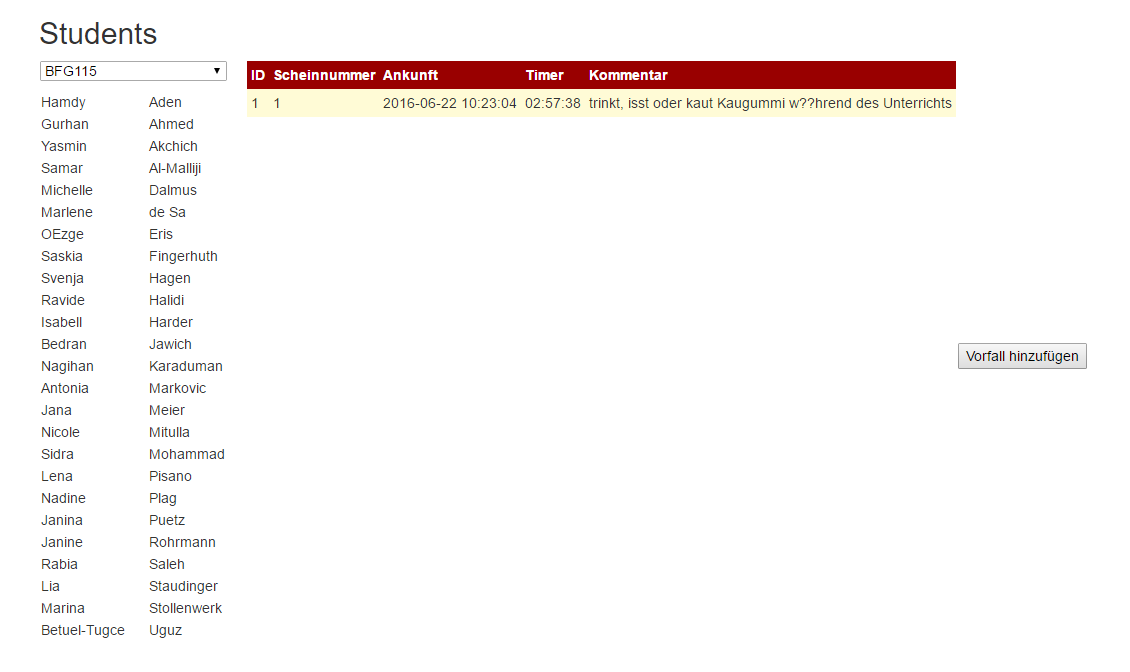
\includegraphics[width=0.9\linewidth]{grafx/webclient}
 \caption[design_webclients]{Design des Webclients}
  \label{fig:webclient_design}
\end{minipage}
\end{figure}
Abbildung  \ref{fig:webclient_design} zeigt das grundlegende Design des
Webclients. Links wird eine Liste mit Klassen und Sch�lern angezeigt und in
der Mitte die Vorfallsliste.\\
Die Vorfallsliste wurde technisch mit einer GridView umgesetzt, die dynamisch
Daten nachladen kann ohne die gesamte Seite zu aktualisieren. So k�nnen per AJAX
Daten nachgeladen werden, ohne das der Benutzer davon etwas merkt.
Anderweitige Funktionen wie das Anlegen eines Incidents oder das Entlassen von
Sch�lern aus dem Trainingsraum wurden bis jetzt nicht umgesetzt, sind aber mit
den vorhandenen Funktionen einfach umsetzbar.
